\section{Methods}

\subsection{MABE}\label{mabe}

In this work, we use the Modular Agent-Based Evolver\cite{bohm_mabe_2017} (MABE) framework to build and run our experiments. MABE allows for the quick construction of agent-based evolution simulations by allowing the scientist to reuse aspects of the system that have already been built by other members of the MABE community. In our work, we use the modules for Markov Brains, Circular Haploid Genomes, simple mutation-only reproduction via roulette selection, and population data archiving. Our programming effort is therefore minimized to simply creating the world module, the module that defines the environment the agent will be evaluated in.

\subsection*{Markov Brains}

We used Markov brains in this work as the evolved controller of our agents. The Markov brains used here consist of four major components: The input vector, output vector, hidden vector, and logic gates. The first three components are simply vectors of values, typically bits, that the gate components can read from and write to. The size of the input, output, and hidden vectors must be decided before the brain is built. The sizes of the input and output vectors are determined by the world module (Section \ref{world}). The size of the hidden vector is independent and is a tunable parameter.

The gates of the agent's Markov brain are, typically, binary logic gates whose input nodes, output nodes, and internal logic are all determined by interpreting the agent's genome. This genome-to-gates interpretation is all handled within MABE's Markov brain module. Gates read from and write to any input, output, or hidden node specified by the genome. Gates can have between 0 and 4 input connections and between 0 and 4 output connections. The smallest functional gate is, therefore, a one-in-one-out gate whose logic can take on 4 unique logic tables. The largest gate possible is a four-in-four-out gate with 256 potential logic tables.

In this work, we also use trit gates, which work the same as the binary gates described above, with the added benefit that trits can take on a third value, $-1$, which can provide useful down-regulation within the brain. Additionally, the one-in-one-out trit gate capable of 9 logic tables while the four-in-four-out trit gate has 6561.

\subsection {Stigmergy World} \label{world}

The world module in MABE is responsible for defining three key aspects of the simulation: The environment, how the agent senses the environment, and how the agent can change the environment.

\subsection*{Map Generation}

In this work, the environment is an $n\times m$ grid surrounded by a wall and filled with smaller wall segments that create obstructions for the agent to navigate around. In addition, the environment contains one home location, where the agent will begin each simulation, and a food location. The environment is constructed by first generating a maze and then removing walls until the desired density of obstacles is reached (Figure \ref{fig:world_explanatory}). This method was chosen to ensure that home and food locations are always reachable by some path through the obstacles.

\begin{figure}
\begin{center}
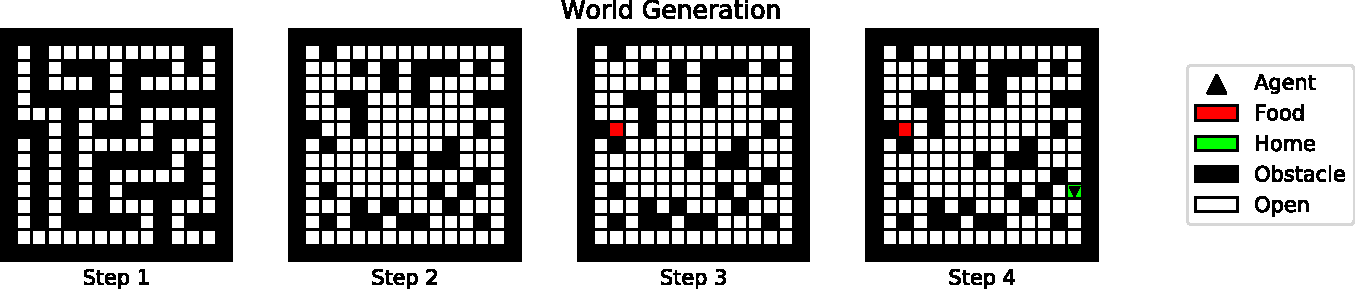
\includegraphics[width=\textwidth]{img/world_explanatory}
\caption{
Caption TODO
}
\label{fig:world_explanatory}
\end{center}
\end{figure}


The maze layout, walls removed, home location, and initial food location are all generated/chosen randomly during environment construction. A new environment is created before every agent evaluation. Furthermore, the location of food may change during an agent's lifetime according to the rules for food use (see Fitness Function). When the food must move, it is randomly relocated.

\subsection*{Agent Inputs}

The agent is equipped with a total of $43+k$ bits of sensor data (Figure \ref{fig:sense_explanatory}). The agent has a vision cone that covers 8 cells with the capability of distinguishing 4 environmental states at each location (32 bits), a $3\times 3$ stigmergy proximity sensor centered on the agent's location (9 bits), an internal compass that provides a two-bit representation of the four cardinal directions, and a stigmergy read sensor that senses the $k$ bit stigmergy signal. In this work we have set $k$ to be $1$, disallowing the agent access to multiple, distinguishable, stigmergy signals. The agent receives input from each of its sensors at every world update.

\begin{figure}
\begin{center}
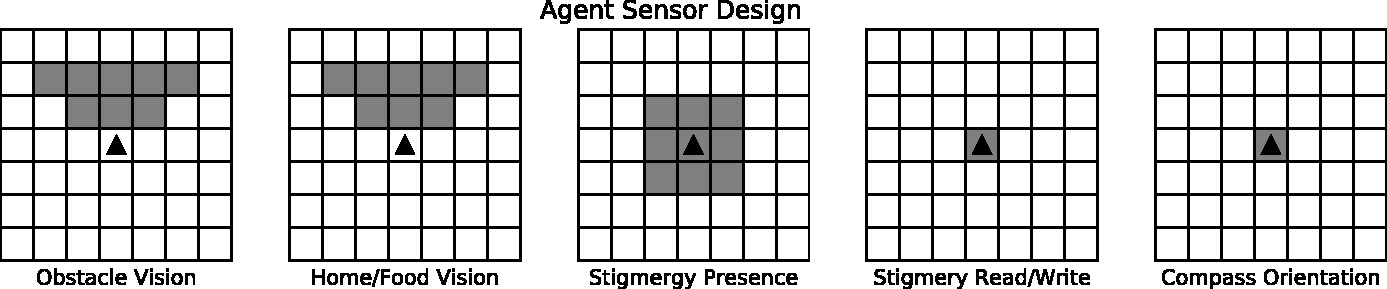
\includegraphics[width=\textwidth]{img/sense_explanatory}
\caption{
The agent's sensors' ranges of influence are indicated by the shaded locations. Left to Right: Agent vision cone wall, food, and home components; Agent pheromone proximity sensor; Agent pheromone secretion and discrimination location; and agent compass.
}
\label{fig:sense_explanatory}
\end{center}
\end{figure}


\subsection*{Agent Outputs}

The agent has a total of $2+k$ output bits. The agent moves throughout the environment via tank controls (Figure \ref{fig:movement_explanatory}) (2 bits). The agent can make no movement by outputting $00$ to the movement bits. The agent also writes $k$ bits to the current location in the form of a stigmergy signal. Writing all zeros is the same as writing no signal. The agent will always output signal on every world update, however, it can choose to do nothing by writing zeros to the move bits, stigmergy bits, or all output bits. Recall that we have set $k$ to be $1$ in this work, so the agent can only write a single kind of signal or write no signal.

\begin{figure}[!htbp]
\begin{center}
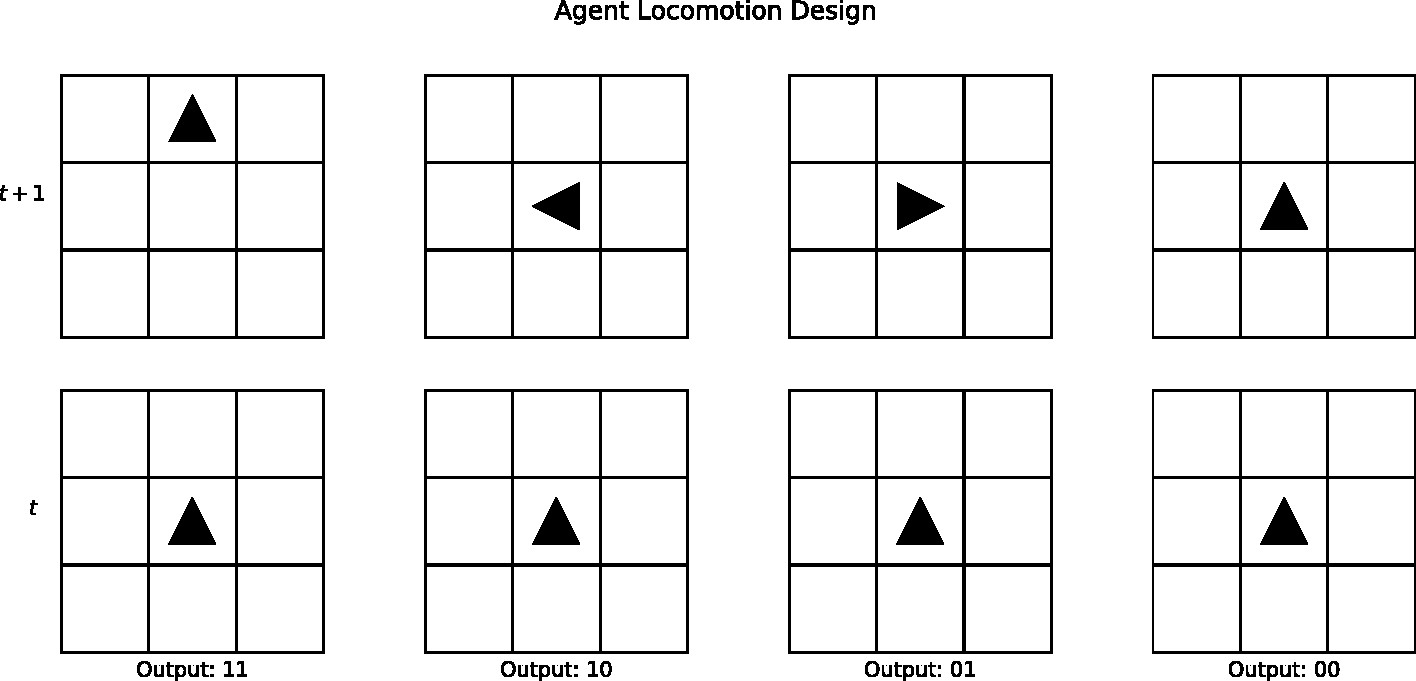
\includegraphics[width=\textwidth]{img/movement_explanatory}
\caption{
Caption TODO
}
\label{fig:movement_explanatory}
\end{center}
\end{figure}


\subsection*{Agent Fitness Function}

During its lifetime (1000 world updates), each agent is tasked with foraging for food, indicated by the food marker on the grid, and returning to the home location with some of it. Each time the agent picks up a piece of food, by stepping on the food location, it adds $+1$ to its fitness. If the agent successfully returns home with the food in hand, the agent adds $+10$ to its fitness. The food location will provide food to the agent a random number of times, between 5 and 10, and then change location on the map. The agent who can quickly locate food, and efficiently make trips between the food and its home, will achieve the highest fitness. Furthermore, each time the agent takes a step forward or places a stigmergic pheromone, the agent receives $+0.001$ fitness. Over the course of the agent's lifetime, these minor fitness payouts can sum to no greater than $2$ points. These small fitness payouts are there to encourage agents to use their outputs and begin walking or secreting pheromone early in the evolutionary run but are kept small enough that once an agent is capable of scoring points from foraging these minor payouts will be negligible to selection.

\subsection {Experimental Design}

<<<<<<< 73926cdf1d134b50d8e6ff9972dcca6f9c50e195
Our goal with this work is to investigate how pheromone evaporation rate affects the fitness of evolved foraging strategies and the degree to which these evolved strategies depend on stigmergy. We hypothesize that evaporation rates that are too extreme, either too slow or too fast, will have low fitness and put selective pressure against the use of stigmergy.
=======
Our goal with this work is to investigate how pheromone evaporation rate affects the fitness of evolved foraging strategies and the degree to which these evolved strategies depend on stigmergy. We hypothesize that evaporation rates that are too extreme, either too slow or too fast, will have low fitness and reduce selective pressure on the use of stigmergy.
>>>>>>> Updates from ShareLaTeX

To test this hypothesis, we first explore the parameter space of our world to determine where agents evolve the fittest strategies without stigmergy. We then use these parameter values to conduct the final experiment with stigmergy. This is done to help mitigate the possibility that stigmergic strategies evolve primarily due to a fundamental limitation on the agent's ability to solve the problem without it.

All agents are evaluated five times in a generation and their scores from these five evaluations are averaged and reported as the agent's fitness for that generation. This is done to help ensure that agents who are placed in an environment that is exceedingly complimentary to their current strategy do not benefit from this lucky event. Rather, agents must have a strategy that is fit, on average, in 5 different environments, reducing the probability of fixation of lucky but generally unfit agents.

\subsection*{Obstacle Density}

As discussed in section \ref{world}, the environment is generated by first building a maze and then randomly removing walls. The percentage of walls that are removed can be varied between 0.00, or a complete maze, and 1.00, an empty $n-1 \times m-1$ grid surrounded by walls. We evolve our agents in environments characterized by 0.00, 0.20, 0.40, 0.60, 0.80, and 1.00 percent wall removal.

\subsection*{Agent Memory}

As discussed in section \ref{mabe}, we used the Markov Brain MABE module to control our agents’ behavior. Markov brains can have any number of hidden nodes which provide the brain with the capability of internal memory. However, too few hidden nodes might make the agent incapable of evolving a fit strategy to a complex problem like stigmergy world, yet too many can make the process of evolution far too slow to do meaningful science. Therefore, we evolve agents that have 0, 1, 2, 4, 8, 16, 32, 64, and 128 hidden nodes to determine where agents are most fit.

\subsection*{Stigmergic Chemical Evaporation Rate}

With the previous two tests completed, we conduct our main experiment to determine how pheromone evaporation affects evolved foraging strategies and to what degree these strategies depend on the use of these pheromones as stigmergic signals. The pheromone evaporation rate is given in units of world updates. We evolved agents with evaporation rates of 1000, 500, 100, 50, 10, 5, and 1. The evaporation rate of 1000 corresponds to permanent pheromone placement, and 1 corresponds to immediate evaporation.

\subsection*{Implementation}

The code used to perform and analyze our experiments, our figures, data from our experiments, tutorials describing how to repeat our experiments and analyses, and video demonstrations of evolved agent behaviors are available via the Open Science Framework at \url{https://osf.io/ydtvs/}.
Each 20,000 generation evolutionary replicate ran approximately four hours on a single-core compute node.
In total, experiments reported consumed roughly 16,000 compute hours.
